\section{Floquet LLs in Dirac systems}
Dirac electrons can be represented with a generic model Hamiltonian like 2D graphene monolayer,

\begin{equation}\label{eq:HDirac}
	\ham_0 =v_F(\sigma _{x}p_{x}+\sigma _{y}p_{y}),
\end{equation}%
where $\vec{p} \rightarrow \vec{p}+e\vec{A}(t)$, here $\vec{A}$ is the vector
potential, $\vec{p}$ is the momentum operator, $v_F$ is the Fermi
velocity of Dirac fermions, $e$ is electron charge,
and $\vec{\sigma}$ the Pauli matrices vector in 2D.
We have two linearly polarized laser lights with the electric field components

\begin{align} \label{eq:EDfield}
\vec{E}_{1} &= E\cos \omega t\ \hat{x}, \nonumber \\
\vec{E}_{2} &= E\cos(Kx)\sin 2\omega t\ \hat{y},
\end{align}
The $\omega $ is frequency of light with time $t$, $K=2\pi /d$ with $d$ being the spatial period of the electric field with
amplitude $E$.
This form of the field leads to the following gauge potential field

\begin{equation}\label{eq:ADirac}
  \vec{A}(t)= \dfrac{E}{\omega} \left\langle -\sin \omega t, \tfrac{1}{2}\cos(Kx) \cos 2\omega t \right\rangle,
\end{equation}%
Substituting Eq.~\eqref{eq:ADirac} into Eq.~\eqref{eq:HDirac}, we arrive at%

\begin{equation}\label{eq:HDtime}
  \ham(t)=\ham_{0} - \sigma _{x} \dfrac{v_F V}{\omega} \sin {\omega t} - \sigma _{y} \dfrac{v_F V}{2\omega}\cos{(Kx)} \cos2\omega t,
\end{equation}%
where $V = eE$.
Because of the time-translation symmetry through $A(t+T)=A(t)$ with $T=2\pi /\omega $, one can apply the Floquet theory \cite{AEE, MBL, supp} and obtain an effective Hamiltonian from Eq.~\eqref{eq:HDtime}.
After performing the Fourier transform of the time-periodicity, first and second order expansion in $\hbar\omega$ terms leads to the final effective Hamiltonian in Eq.~\eqref{eq:HDtime} as

\begin{equation} \label{eq:HDeff}
  \ham_{\text{eff}}=\ham_{0}-\sigma_y\frac{v_F^3 V^2 p_y}{\hbar^{2}\omega^{4}}
  +\sigma_y\frac{v_F^3 V^{3}\cos{(Kx)}}{2\hbar^{2}\omega^{5}}
  -\sigma_x\frac{v_F^3 V^2 \left\{p_x, \cos{(Kx)} \right\} }{8\hbar^{2}\omega^{4}}.
\end{equation}
In Eq. ~\eqref{eq:HDeff}, first order term in $\hbar \omega$ that leads to gap at the Dirac point in usual circularly polarized light experiments \cite{YHW, JWM} is zero here due to inhomogeneous nature of laser lights.
This effective Hamiltonian can be simplified in the long wavelength limit, $Kx \ll 1$ to

\begin{align} \label{eq:HeffB}
  \ham_{\text{eff}} &= v_F \sigma_x p_x + v_F \sigma_y \left[ \left( 1- \dfrac{v_F^2V^2}{\hbar^2\omega^4} \right) p_y + \dfrac{K v_F^2 V^3}{4 \hbar^2 \omega^5} x \right] \nonumber \\
  \ham_{\text{eff}}^D &= v_{F}\sigma_{x}p_{x}+v_F\sigma_{y} \left( C p_{y} + qB^Dx \right)
\end{align}%
In obtaining Eq.~\eqref{eq:HeffB}, last term in Eq.~\eqref{eq:HDeff} is second order in space and thus zero in the long wavelength limit for the spatially inhomogeneous modulation.
Further, we have $B^D=\frac{Kv_F^2 e^2E^3}{4\hbar^{2}\omega^{5}}$.
In accordance with Eqs.~\eqref{eq:HDeff} and ~\eqref{eq:HeffB}, there is least anisotropy in the Dirac spectrum in addition to zero gap.
Diagonalizing the Hamiltonian in Eq.~\eqref{eq:HeffB}, we obtained the eigenvalues for Dirac system as%

\begin{equation} \label{eq:DiracEner}
  \epsilon_{n}^D = \pm v_F^2 \sqrt{\dfrac{nK e^3 E^3}{2 \hbar \omega^5}}
\end{equation}
which is similar to graphene LLs spectrum in the limit of equal velocities.
We can have gapped Dirac spectrum by using uniform circularly polarized laser light as observed in experiments \cite{YHW, JWM} or by using any substrate like hBN.
It is also important to note that the effective magnetic field strength obtained for Dirac case in Eq.~\eqref{eq:DiracEner} is directly proportional to third order of the electric field and inversely proportional to the product of spatial period and fifth order of the frequency of the polarized light $\propto (E^3/(d\omega^5))$.
This factor of the laser lights can be tuned and thus effective magnetic field can be enhanced in such nonequilibrium systems.

\subsection{Dirac numerical approach}

\begin{figure}[h]
  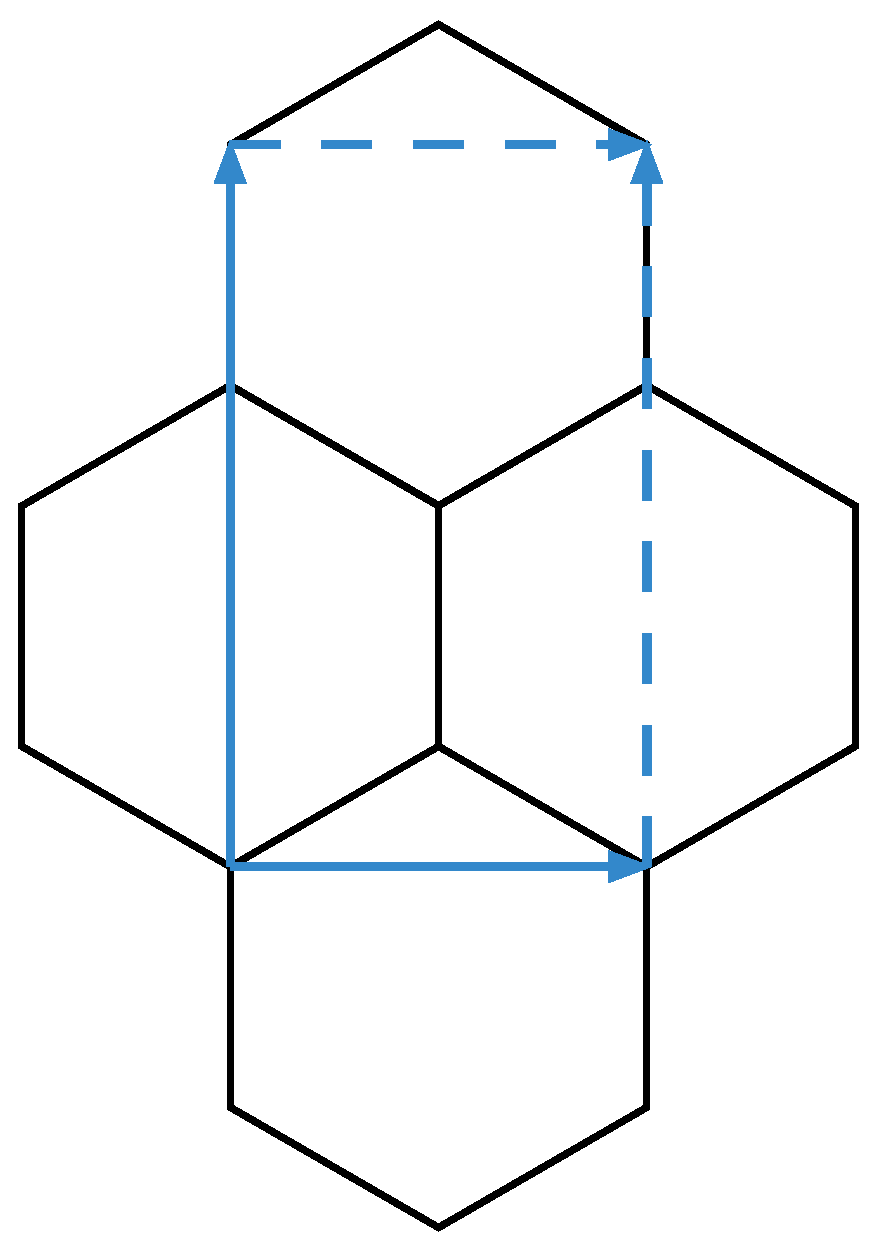
\includegraphics[width=0.33\textwidth]{./figures/dirac-floquet-unit-cell.pdf}
  \caption{Honeycomb lattice depicting 4 atoms per unit cell for inhomogeneous incident laser light.}
  \label{fig:honeycomb}
\end{figure}

We now look beyond perturbation theory.
In doing so we will have to solve the system numerically, which we will describe next.
The incident laser light doesn't allow for translation symmetry along the x-axis for our Dirac honeycomb system.
We consider a simple model using 4 atoms in a unit cell, the lattice vectors are $\vec{a}_1 = \sqrt{3}a\hat{x}$ and $\vec{a}_2 = 3a\hat{y}$, as can be seen in figure \ref{fig:honeycomb}.
Our Hamiltonian takes the following form

\begin{equation}
  H = -\sum_{j'l'\alpha,jl\beta} h^{j'l'\alpha}_{jl\beta} C^{\dagger}_{j'l'\alpha} C_{jl\beta} + h.c.,
\end{equation}
where $t$ is the hopping amplitude, $j,l$ are unit cell index in x and y, and $\alpha,\beta = A_1, A_2, B_1, B_2$.
To include the vector potential from Eq.~\eqref{eq:ADirac} in the tight-binding model we consider a finite system defined by $r_c \geq \max(|x_{i\alpha}|,|y_{i\beta}|)$.
Using a Peierls substitution we can write the hopping term as

\begin{align}
h^{j'l'\alpha}_{jl\beta} &= h \exp\left[ i \phi_0 \left\{ (x_{j'l'}^{\alpha} - x_{jl}^{\beta}) \sin{\omega t} - \dfrac{1}{2} \sin\left(K \dfrac{x_{j'l'}^{\alpha} + x_{jl}^{\beta}}{2} \right) (y_{j'l'}^{\alpha} - y_{jl}^{\beta}) \cos{2\omega t}  \right\} \right] \nonumber \\
  &= h \exp\left[ i X_1 \sin{\omega t} -i X_2 \cos{2\omega t}\right]
\end{align}
where $ $.
One can fourier transform along the y-axis to momentum space to simplify our system to

\begin{equation}
  H = -\sum_{jk} \left[ \Psi^{\dagger}_{jk} H_{j,j} \Psi_{jk} + \Psi^{\dagger}_{j,k} H'_{j,j+1,k} \Psi_{j+1,k} + h.c. \right],
\end{equation}
where $\Psi_{jk} = [C_{jkA_1}, C_{jkB_1}, C_{jkA_2}, C_{jkB_2}]^T$. The two matrices are
%\[
%  H_{j,j} =
%  \begin{bmatrix}
%    0 & t^{jlA_1}_{jlB_1} & 0 & 0 \\
%    t^{jlB_1}_{jlA_1} & 0 & t^{jlB_1}_{jlA_2} & 0 \\
%    0 & t^{jlA_2}_{jlB_1} & 0 & t^{jlA_2}_{jlB_2} \\
%    0 & 0 & t^{jlB_2}_{jlA_2} & 0
%  \end{bmatrix}
%\]
\[
  H_{j,j} =
  \begin{bmatrix}
    0 & 0 & 0 & 0 \\
    t^{jlA_1}_{jlB_1} & 0 & 0 & 0 \\
    0 & t^{jlB_1}_{jlA_2} & 0 & 0 \\
    0 & 0 & t^{jlA_2}_{jlB_2} & 0 \\
  \end{bmatrix}
\]
and
\[
  H'_{j,j+,k} =
  \begin{bmatrix}
    0 & t^{j+1,lA_1}_{jlB_1} & 0 & t^{j+1,l+1,A_1}_{jlB_2} e^{i\vec{k}\cdot\vec{a}_2} \\
    0 & 0 & 0 & 0 \\
    0 & 0 & 0 & t^{j+1,lA_2}_{jlB_2} \\
    0 & 0 & 0 & 0
  \end{bmatrix},
\]
where $\vec{k} = k \hat{y}$.
The Hamiltonian dimension is reduced to $N_S \times N_S$, with $N_S = 2r_c+1$.

For Floquet theorem we next consider how to construct the Quasienergy operator $\bar{Q}$.
We first need to calculate the fourier time transform of our Hamiltonian.
Each component of the matrix can be written as the following

\begin{align}
  H_{ab, n} &= \dfrac{1}{T} \int^T_0 H_{ab} e^{-i n \omega t} dt \nonumber \\
  &= \dfrac{1}{2\pi} \int^{2\pi}_0 e^{iX_1\sin{\tau} - iX_2\cos{2\tau} - i n \tau} d\tau.
\end{align}
This integral form is close to a Bessel function but has no elementary solution thus we solve it numerically.
The quasienergy matrix $\bar{Q}$ then has matrix elements

\begin{equation}
  \bar{Q}_{m,m+n} = H_n - m \hbar \omega \delta_{n0}
\end{equation}
We choose a cutoff for mode m, $|m| \leq m_c$, where $m_c$ is a positive integer.
This means we will have $N_m = 2 m_c +1$ diagonal blocks, where each block is a $N_S \times N_S$ matrix, $H_n$.

